\documentclass[a4paper]{article}

%% Language and font encodings
\usepackage[english]{babel}
\usepackage[utf8x]{inputenc}
\usepackage[T1]{fontenc}

%% Sets page size and margins
\usepackage[a4paper,top=3cm,bottom=2cm,left=3cm,right=3cm,marginparwidth=1.75cm]{geometry}

%% Useful packages
\usepackage{amsmath}
\usepackage{graphicx}
\usepackage[colorinlistoftodos]{todonotes}
\usepackage[colorlinks=true, allcolors=blue]{hyperref}
\usepackage{float}
\usepackage{enumerate}
\usepackage{subfig}

\title{A cursory search engine : ASBS}
\author{2019201411}

\begin{document}
\maketitle

\section{Introduction} ASBS is a in-station search engine. It can be used for search function in some small site, like Info school of RUC. And it works as many pouplar search engine, it gets the input information and find the Top 10 websites which are best matches to display. However, it is built by home server. So you can only used it when you download the whole project and built it in proper order. What's more, it's small-scale. So it may be broken down when you use it to deal with a huge station. \textbf{All of the content is only for scientific research.}

\section{Details}
\subsection {Crawl}
I use the "wget" command in C++ to download the html of the sites. A disadvantage is that I don't use multithread processing so that I set the sleep time as 1s. And it will take 2h to get all pages belonging to http://info.ruc.edu.cn.

\subsection {HTML parser and word-seg}
\begin{enumerate}[i)]
\item I view the files downloaded by wget as some "txt", and I extract the content which has label <p> or <title>.
\item As to word-seg, I use jieba-py to cut the words. 
\end {enumerate}

\subsection {Scoring}
To choose the best mathes, we need to assign a score to each site. We assume that we have N docs(or html of sites).
\begin{itemize}
\item First we define $tf_{t,d}$ as the occur times of term $t$ in doc $d$.
\item And then we define $df_{t}$ as the number of docs which we can find term $t$ in them.It means if $t$ occurs many times in a doc,it will only be counted once.
\end{itemize}
Define 
\[W_{t,d}=(1+log_{10}tf_{t,d})*(log_{10}N/df_{t})\] 
\par
And for a certain query, we calc $W_{t,q}$ as above. To calc the similarity between the query and the docs, we view query and docs as same-order vectors($W_{d}, W_{q}$), and the dimension is decided by the num of terms in query. We regard the angle between 2 vevtors as the similarity. Closer they are, we suppose they are more similar. So we use the cosine to calc the final Score.
\par
But when we test a few queries, we find that somtimes it doesn't perform well. Considering that the titles really means a lot, so I give the term in the title more weight.

\subsection{UI}
\begin{itemize}
\item Use flask to communicate between server and user.
\item Simple css to build the html. 
\end{itemize}

\section {Some tricks}
Actually they are some problems when coding, I've mentioned them in the presentation. By the way, to strong the key words occur in the abstract in the result-website, I add <strong></strong> around the key word, it's kind of silly but really easy and efficient.

\section {Display}
\begin{description}
\item[Advantages] For those news query, ASBS usually get satisfactory results. Because the news report are unique in generally. And if the query is compose of few words, always good answers.
\item[Disadvantages] Since I did not set the stop words, so when the input has the similar meaning with the passage but not same or the query has so many key word, then the results may not be that satisfying.
\end{description}
\begin{figure} [H]
 \centering
  \subfloat[homepage]{
   \label{f:(a)}
    
\includegraphics[width=0.3275\textwidth]{homepage.png}}
  \subfloat[result1]{
   \label{f:(b)}
    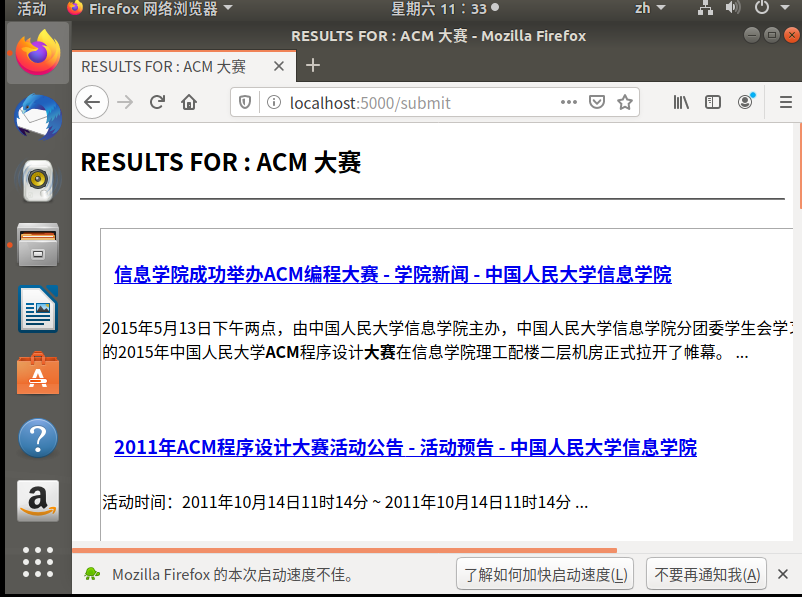
\includegraphics[width=0.3275\textwidth]{res1.png}}
  \subfloat[result2]{
   \label{f:(c)}
    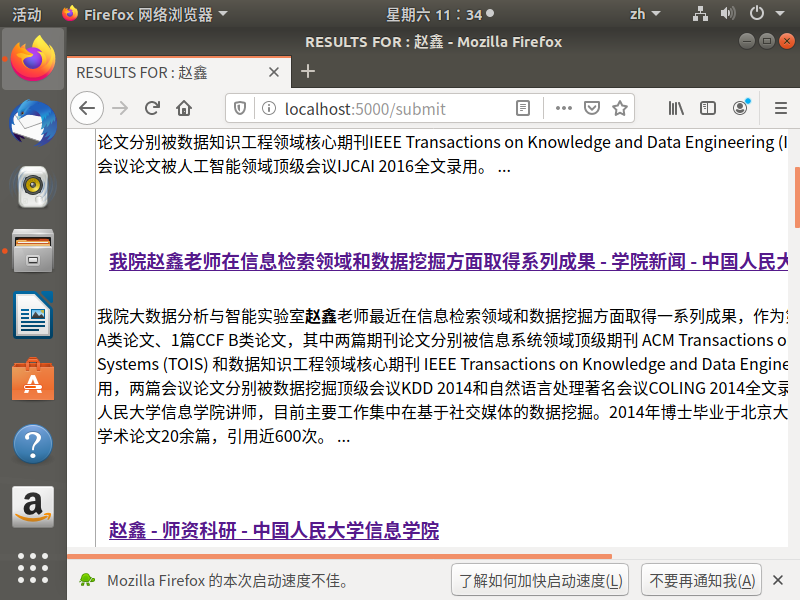
\includegraphics[width=0.3275\textwidth]{res2.png}}
 \caption{pictures about ASBS}
 \label{f:pictures about ASBS}
\end{figure}
In conclusion, I use C++ and python to bulid this task. It's really challenge for me since that I have some problems in C++ web programming and turn to using python(start from very beginning). However, I really learned a lot from it and it's an interesting project that I will continue to solve the problem which I encountered before(the calculate method and use C++ to finish the task). Really a good way to kill time in summer vacation. And thanks for Professor Zhao xin, and TA Menci.
\section*{Appendix : How to use ASBS}
\appendix
\textbf{Requirements:}python3.0+, Ubuntu
\section{pretreat}
\begin{enumerate}[i)]
\item edit crawl.cpp and modify ROOTURL. The default ROOTURL will be http://info.edu.ruc.cn/
\item edit crawl.cpp and modify the sleep time.
\end{enumerate}
\section{run}
\begin{enumerate}[i)]
\item crawl.cpp, analyze.cpp, test.cpp, app.py, templates should be in the same catalogue.
\item compile and run crawl.cpp, analyze.cpp, test.cpp in order. And you will find a number output on the shell, memorize the number as N. Use "python app.py -num N" to run. And the homepage will be "localhost:5000/submit".
\end{enumerate} 
\end{document}